\section{Cipher Specifications}
\setbeamercovered{transparent}
\begin{frame}{Description of PRINCE}
\begin{enumerate}
    \item PRINCE is a 64-bit block cipher with a 128-bit key consisting of 12 rounds
    \pause
    \item The key is split into two
parts of 64 bits each i.e. k = k0$||$k1
     \pause 
     \item Another part of the key $k_0'$ is derived from $k_0$ by using the following relation 
     $k_0' = (k_0 >>> 1) \bigoplus (k_0 >> 63)$
     \pause
     \item The keys $k_0$ and $k_0'$ are used are whitening keys and the key $k_1$ is used as the round key for the core function. \\
     \pause
     \item 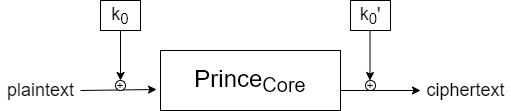
\includegraphics[scale=0.5]{Cipher.jpg}
\end{enumerate}


\end{frame}

\begin{frame}{Rounds of Prince}
\begin{enumerate}
    \item PRINCE consists of 12 rounds which include the following :
    \begin{enumerate}
        \item First 5 rounds or the "forward rounds"
        \item The middle round which is termed as 2 rounds
        \item The last 5 rounds or the "backward rounds"
    \end{enumerate} 
 
\end{enumerate}.  \\ \\ \\ \\
      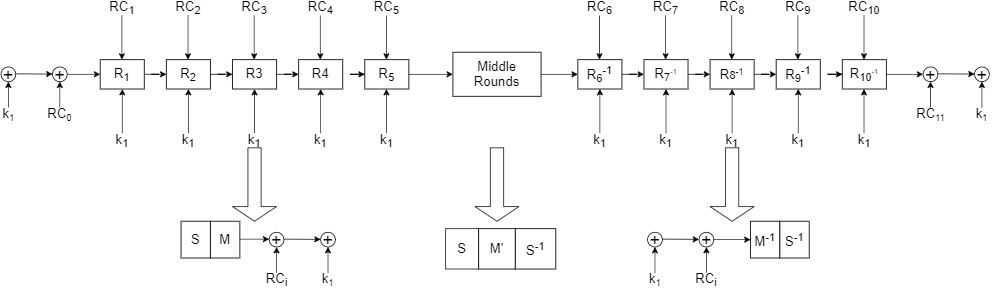
\includegraphics[scale=0.45]{Prince-12-Round.JPG}
\end{frame}

\begin{frame}{Specifications of Prince}
\begin{itemize}
    
    \item S-Layer :- Prince uses a 4-bit S-box. It is as follows : \\
     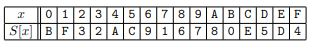
\includegraphics[]{S-box.JPG} \\ \\
     \item Linear Layer :- This layer provides diffusion. It is a combined layer consisting of a shift row followed by a 64 $\times$ 64 matrix multiplication.
     \item Round Constants :- There are 12 round constants from $RC_0$ to $RC_{11}$ such that $RC_i \oplus RC_{11-i} = \alpha$. \\
     Here, $\alpha$ = c0ac29b7c97c50dd \\
     \item Key Addition :- The 64-bit $k_1$ is xored with the state. 
\end{itemize}
\end{frame}

\begin{frame}{Specifications of Prince}
\begin{itemize}
    
   \item The Round Constants Used are as follows : \\
   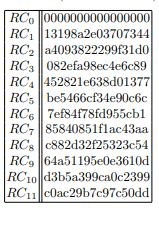
\includegraphics[scale=0.8]{RoundConstants.JPG} \\ \\
\end{itemize}
\begin{block}{$\alpha$ Reflection property}
\begin{itemize}
    \item $RC_i \oplus RC_{11-i} = \alpha$ 
    \item $RC_1$, . . . , $RC_5$ and $\alpha$ have been derived from the fraction part of $\pi$
\end{itemize}
\end{block}
\end{frame}


\begin{frame}{Specifications of Prince}
\begin{itemize}
    
   \item The Linear Layer M consists of 2 parts  : \\
   \begin{itemize}
       \item Shift Rows :- This performs a circular shift operation on the rows similar to that used in AES. The mapping of the Shift Row operation is as follows : \\  \\ \\
       \begin{adjustbox}{width=\linewidth}
       \begin{tabular}{|l|l|l|l|l|l|l|l|l|l|l|l|l|l|l|l|}
            \hline
        0 & 1 & 2  & 3  & 4 & 5 & 6  & 7 & 8 & 9  & 10 & 11 & 12 & 13 & 14 & 15 \\ \hline
        0 & 5 & 10 & 15 & 4 & 9 & 14 & 3 & 8 & 13 & 2  & 7  & 12 & 1  & 6  & 11 \\ \hline
        \end{tabular} \\
        \end{adjustbox} \\ \\
       \item M' Layer :- This is a 64 $\times$ 64 binary matrix representated as follows : \\ 
        $M'=$
      \begin{pmatrix} 
    M_0 & 0 & 0 & 0\\
    0 & M_1 & 0 & 0\\
    0 & 0 & M_1 & 0\\
    0 & 0 & 0 & M_0\\
    \end{pmatrix}
    
   \end{itemize}
\end{itemize}
\end{frame}
\begin{frame}{Specifications of Prince} 
\begin{itemize}

 \item The constituent 16 $\times$ 16 matrices $M_0$ and $M_1$  further contain 4 $\times$ 4 matrices as follows : \\ \\ \\ \\ \\
 \item $\Vec{M^{(0)}}=$
\begin{bmatrix} 
$M_{0}$ & $M_{1}$ & $M_{2}$ & $M_{3}$\\
$M_{1}$ & $M_{2}$ & $M_{3}$ & $M_{0}$\\
$M_{2}$ & $M_{3}$ & $M_{0}$ & $M_{1}$\\
$M_{3}$ & $M_{0}$ & $M_{1}$ & $M_{2}$\\
\end{bmatrix}
\item $\Vec{M^{(1)}}=$
$\begin{bmatrix} 
$M_{1}$ & $M_{2}$ & $M_{3}$ & $M_{0}$\\
$M_{2}$ & $M_{3}$ & $M_{0}$ & $M_{1}$\\
$M_{3}$ & $M_{0}$ & $M_{1}$ & $M_{2}$\\
$M_{0}$ & $M_{1}$ & $M_{2}$ & $M_{3}$\\
\end{bmatrix}$
\end{itemize}
\end{frame}

\begin{frame}{Specifications of Prince}
\begin{itemize}
\item The smaller 4 $\times$ 4 matrices used are as follows : \\
\item     $M_{0}=$
\begin{bmatrix} 
0 & 0 & 0 & 0\\
0 & 1 & 0 & 0\\
0 & 0 & 1 & 0\\
0 & 0 & 0 & 1\\
\end{bmatrix}
\,
$M_{1}=$
\begin{bmatrix} 
1 & 0 & 0 & 0\\
0 & 0 & 0 & 0\\
0 & 0 & 1 & 0\\
0 & 0 & 0 & 1\\
\end{bmatrix}
\\
$M_{2}=$
\begin{bmatrix} 
1 & 0 & 0 & 0\\
0 & 1 & 0 & 0\\
0 & 0 & 0 & 0\\
0 & 0 & 0 & 1\\
\end{bmatrix}
\,
$M_{3}=$
\begin{bmatrix} 
1 & 0 & 0 & 0\\
0 & 1 & 0 & 0\\
0 & 0 & 1 & 0\\
0 & 0 & 0 & 0\\
\end{bmatrix}
\\
\end{itemize}
\begin{block}{Important}
\item \underline{Point to Note}:- The Linear Layer Used in Prince is an involution. This implies that it is its own inverse. This fact helps in symmetric decryption with little to no overhead over the original encryption function.
\end{block}
\end{frame}